%!TEX root = ./memoire/main.tex

\chapter{Evaluation et comparaison des méthodes de correction de position et/ou d'intensité}

\section{Objectifs}

En définissant dans le précédent chapitre un filtre par correction de position, nous proposons\dots

\section{Définition du problème}
\subsection{Problème des trois vortex}

Nous évaluerons les résultats des filtres à l'aide du problème des trois vortex~\cite{aref_motion_1979,yim_motion_2022}. Il s'agit d'un problème analogue au problème à N-corps pour la mécanique céleste. A partir de trois corps, Henri Poincaré a montré que ces problèmes sont sensibles aux conditions initiales, initiant ainsi la théorie du chaos moderne~\cite{poincare1890,diacu1996}.

Chaque tourbillon est positionné sur une boite de taille $[0, \pi]^2$  et suit la distribution du tourbillon de Bessel~\cite{vanGeffen1996}. Un tourbillon de Bessel est défini par un champ de vorticité continu sur un cercke de rayon $R$ et d'équation

\begin{equation*}
    \omega(r) =  \begin{cases}
        \Gamma ~ J_0\left(\frac{k  r}{ R}\right),   \quad & r < R,        \\
        0 \quad                                           & \text{sinon},
    \end{cases}
\end{equation*}où $J_0$ est la première fonction de Bessel, $k$ son premier zero non trivial, $r$ la distance au centre du tourbillon et $\Gamma$ une intensité.

Indépendemment, il s'agit de solution stationnaire pour les équation d'Euler dans un domaine infini. Dans ce cas, chaque vortex tourne autour de son centre, avec une vitesse angulaire constante $\frac{\Gamma}{2\pi}$ sans changer de forme. Lorsque lorsque plusieurs tourbillons sont placés dans une boite, ceux-ci vont commencer à ce déplacer du fait des vitesses induites les uns aux autres et également du fait des conditions limites. La figure~\ref{sec:ref_three_vortex} représente la trajectoire de trois tourbillons au cours du temps.

% Rajouter la configuration des particules initales
\begin{figure}~\label{sec:ref_three_vortex}
    \centering
    \begin{subfigure}{0.5\textwidth}
        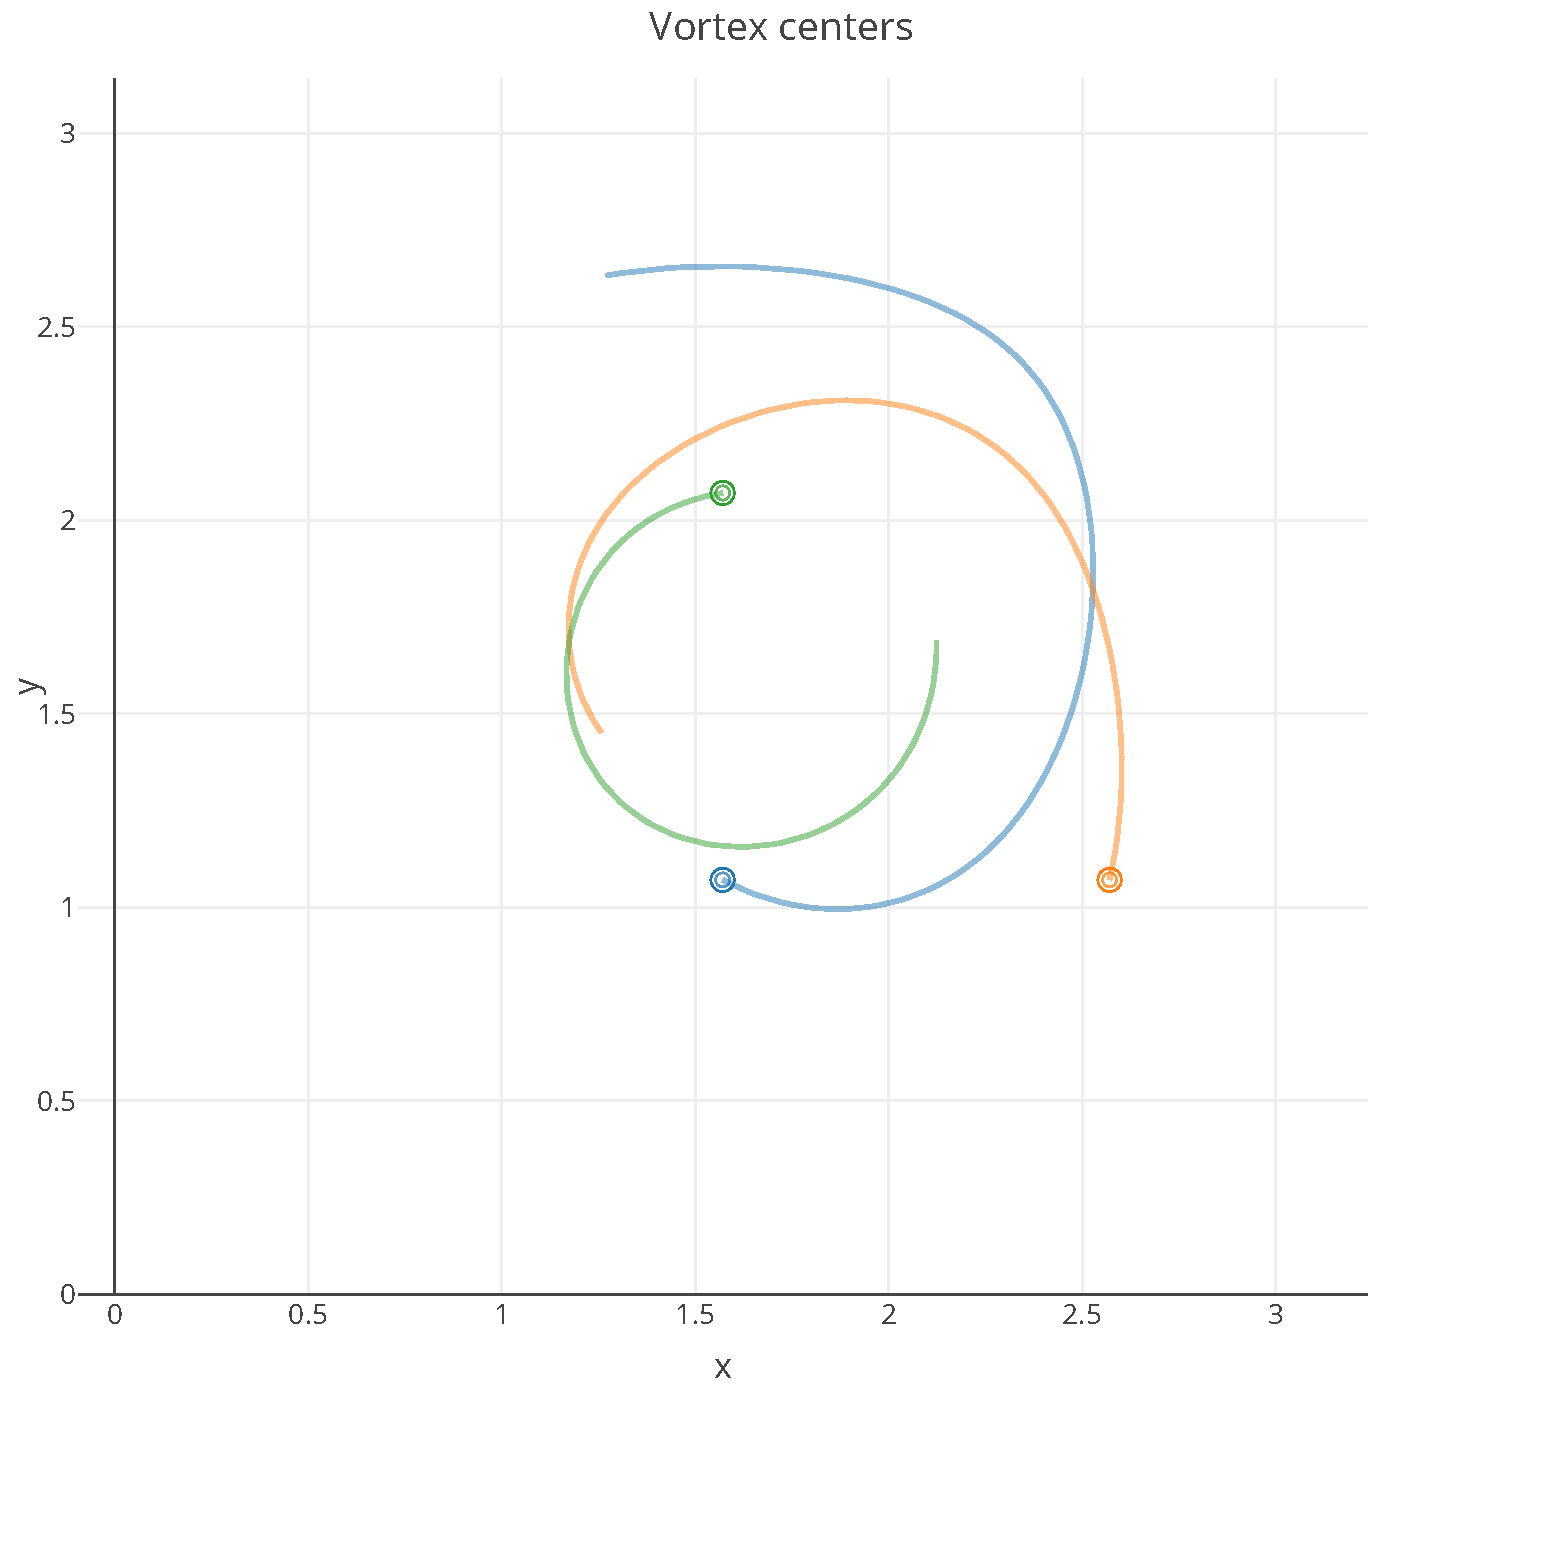
\includegraphics[width=\textwidth]{vortex_centers.pdf}
        \caption{Trajectoire des centres de trois tourbillons au cours du temps.}
    \end{subfigure}
\end{figure}

Les paramètres de cette configuration de référence sont raportés dans la Table~\ref{tab:ref_three_vortex}.

\begin{table}[htbp]
    \centering
    \caption{Paramètre du problème de référence.}
    \begin{tabular}[t]{|l|l|}
        \hline
        Variables              & Distributions                 \\
        \hline
        Centre du tourbillon 1 & $[\pi / 2, (\pi - 1) /2]$     \\
        Centre du tourbillon 2 & $[\pi / 2 + 1, (\pi - 1)/ 2]$ \\
        Centre du tourbillon 3 & $[\pi / 2, (\pi + 1) / 2]$    \\
        Taille de coeur $R$    & 0.2                           \\
        Amplitude $\Gamma$     & 4.0                           \\
        Temps de simulation    & 50.0                          \\
        \hline
    \end{tabular}
    \label{tab:ref_three_vortex}
\end{table}

\subsection{Assimilation du centre des vortex}

Du fait du caractère chaotique du problème, une faible perturbation dans les conditions initiales entraine une amplification de l'erreur sur les trajectoires de tourbillon. Nous supposons initialement que le centre des tourbillon, leur taille $R$, et leur amplitude $\Gamma$, sont connus avec une incertitude initiale dont les valeurs sont rapportées dans la Table~\ref{tab:init_three_vortex}. A
L'objectif dans cette section sera donc de faire le suivi de la position des trois vortex.

\begin{table}[htbp]
    \centering
    \caption{Conditions initiales}
    \begin{tabular}[t]{|l|l|}
        \hline
        Variables             & Distributions                                                        \\
        \hline
        Centre du tourbillon  & $\mathcal N(x^i,0.05), \quad \mathcal N(y^i,0.05) \quad i = {1,2,3}$ \\
        Taille de coeur ($R$) & $\mathcal N(0.2, 0.01)$                                              \\
        Amplitude ($\Gamma$)  & $\mathcal N(4.0, 0.08)$                                              \\
        \hline
    \end{tabular}
    \label{tab:init_three_vortex}
\end{table}


